\documentclass[addpoints,12pt]{exam}
%\documentclass[12pt]{article}
\usepackage[letterpaper, margin=0.75in]{geometry}
\usepackage{graphicx}
\usepackage{enumitem}
\usepackage{booktabs}
\usepackage{tabularx}
\usepackage{amsmath}
\usepackage{color}

\begin{document}
\footer{}{Page \thepage\ of \numpages}{}

\begin{flushright}
\makebox[0.5\textwidth]{\large Name:\enspace\hrulefill}
\vspace{0.2in}

\makebox[0.5\textwidth]{\large Date:\enspace\hrulefill}
\end{flushright}

\begin{center}

\includegraphics[width=10cm]{../images/logo.png}
\end{center}

\begin{center}
\noindent{\LARGE Conceptual Physics \\ Homework Packet 3\\}
\end{center}
\noindent\begin{large}\textbf{Due: March 23, 2018}\end{large}
\vspace{0.2in}

Answer the questions in the spaces provided on the question sheets. If you run out of room for an answer, continue on the back of the page. If questions are taken from one of the textbooks, it will be indicated. A large portion of your grade will be calculated based on \textit{how} you obtained an answer, so please \textbf{show your work} (including all diagrams and drawings if relevant).

If you prefer working on loseleaf paper, or have a large portion of your work on loseleaf, please be sure to hand that in along with this homework packet.

The content in this homework relates to material we covered in class 4 (forces) and class 5 (energy). The related readings are:
\begin{enumerate}
	\item Handout on \textit{The Fundamental Interactions} in the course reader.
	\item \textit{Light and Matter}, Chapter 4 (all Sections)
	\item Handout on \textit{Conservation of Mass and Energy} in the course reader. (All sections except 3)
	\item \textit{Light and Matter}, Chapter 13 (Section 1)
	\item \textit{College Physics}, Chapter 7 (Sections 1 to 6)
\end{enumerate}

Below is a cartoon picture of the atom, following the atomic model that makes it look like planets:

\noindent \begin{center}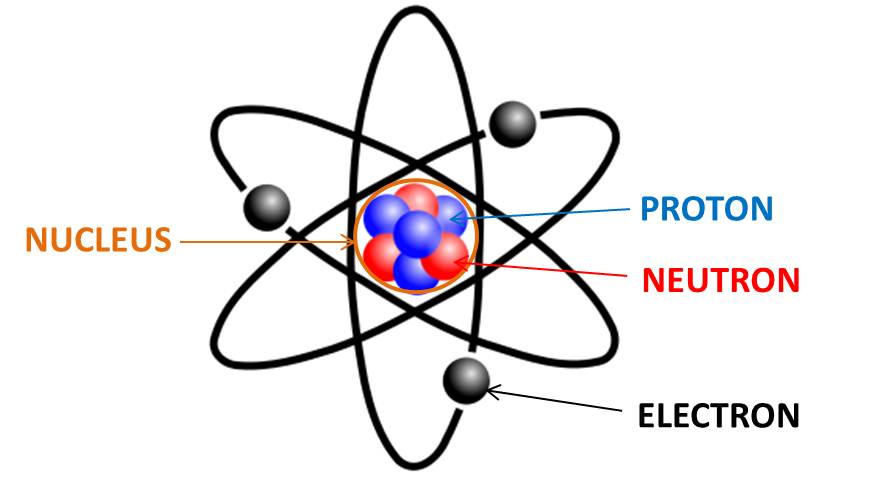
\includegraphics[width=4in]{../images/atom.jpg}\end{center}

Where the \textit{nucleus} is located in the middle of the atom and is orbited by electrons. Protons are \textit{POSIT}ively charged, neutrons carry no charge (\textit{NEUT}ral) and electron are negatively charged (and named for archaic reasons having to due with Greeks and tree resin). Electrons are \textit{fundamental particles} - they cannot (to our knowledge) be further broken down. Protons and neutron, however, are composite particles, meaning that they can be further broken down. \textit{Quarks} come together to form protons and neutrons, and are themselves fundamental particles (discussed in Chapter 0 of \textit{Light and Matter} and chapter 33, section 5 of \textit{College Physics}).

 
\clearpage

\begin{flushright}
Score: \hspace{0.2in} / \numpoints ~ points
\end{flushright}


\begin{questions}
\question[4] 
\begin{parts}
\part 
Why do people mostly notice the gravitational force acting on their bodies if it is such a comparatively weak force?
\fillwithlines{1.5in}

\part In what ways, if any, do we notice the other forces?
\fillwithlines{1.5in}
\end{parts}
	
	\question[4]
	Two satellites are orbiting the Earth. Satellite A has a mass of 100~kg, satellite B has a mass of 200~kg. If they are orbiting at the same distance from Earth, which (if any) experiences the greater gravitational force? Why? (I recommend you draw a diagram - but it's optional)
		\vspace{1.5in}
		
	\question[4]
	The Apollo spacecraft felt gravitational attractions from both the earth and the moon. Was there any time during the flight when \textbf{one} of these forces was zero? Could a place exist where the \textbf{net} force from the earth and the moon was zero? (From \textit{The Fundamental Interactions} handout, problem B4)
		\vspace{1.5in}
	 
	\clearpage
\question[6]
	Tides arise from gravitational interactions between the Earth and the Moon. (\textit{High tides} are the state of the tide when at its highest level.) Because the Moon rotates about the Earth once every 28 days, the high tides to not occur at the same time each day. Also, the magnitude of the high tide will vary from day to day. To understand why, consider the positions of the Moon relative to the Sun and Earth below:
	\begin{center}
	\input{../images/hightides.pdf_tex}
	\end{center}
	\begin{parts}
		\part For which of these configurations will the high tide be the greatest? Please explain.
			\vspace{1.5in}
		\part For which of these configuation with the high tide be the least? Please explain.
			\vspace{1.5in}
		\part Describe the Sun's role in determining the magnitude of the high tides.
			\vspace{1.5in}
	\end{parts}
	
	\clearpage
		
	\question[4]
	\begin{parts}
		\part You release a magnet on a tabletop near a big piece of iron, and the magnet leaps across the table to the iron. Does the \textbf{magnetic potential energy} increase, or decrease? Explain.
		\vspace{1.5in}
		\part Suppose instead that you have two repelling magnets. You give them an initial push towards each other, so they decelerate while approaching each other. Does the \textbf{magnetic potential energy} increase, or decrease? Explain.
		\vspace{1.5in}
	\end{parts}

\bonusquestion[4]
	You jump straight up in the air.
	\begin{parts}
		\part When do you have the greatest gravitational potential energy? When do you have the greatest kinetic energy?
			\vspace{2in}
		\part Assume your mass is 70~kg and you reach a maximum jumping height of 1.25~m. Prove that your initial velocity must have been at least 5~m/s up. (let $g = 10~m/s^2$. If you don't have a calculator, it may be easier to write 1.25~m as 5/4~m)
			\vspace{2in}
	\end{parts}	


\end{questions}








\end{document}